\section{Mathematical model} \label{sec:model}

First of all, it is necessary to introduce a fixed inertial reference frame $\{  \textbf{e}_1,  \textbf{e}_2,  \textbf{e}_3  \}$ and a body-fixed frame $ \{  \textbf{b}_1,  \textbf{b}_2,  \textbf{b}_3 \}$. Next, we present
a general equation for calculating CoG vector from the origin of the body-fixed frame as follows: 
\begin{equation}
	\textbf{r}_{CoG} = \frac{m_{b}\textbf{r}_{b} + \sum_{i=1}^n m_{i} \textbf{r}_{i}}{m_{b} + \sum_{i=1}^n m_{i}} = \frac{\sum_{i=1}^n m_{i}\textbf{r}_{i}}{m_t},
	\label{equ:cog}
\end{equation}

The following terms are defined as: \todo{1.1 a)}
\begin{itemize}
	\item $ \textbf{r}_{CoG} \in \mathbb{R}^3$ - CoG with respect to the body-fixed frame
	
	\item $ \textbf{r}_{i} \in \mathbb{R}^3$ - Position of the i-th mass or payload w.r.t. the body-fixed frame
	
	\item $ \textbf{r}_{b} \in \mathbb{R}^3$ - Position of UAV body w.r.t. the body-fixed frame. Note that because the body frame origin coincides with the rigid body CoG (without considering the moving masses) this term yields $ \textbf{r}_b = 0_{3x1}$
	
	\item $m_b \in \mathbb{R}$ - Mass of the UAV body 
	
	\item $m_i \in \mathbb{R}$ - Mass of the i-th moving mass or payload
	
	\item $m_t \in \mathbb{R}$ - Mass of the whole UAV system
\end{itemize}

Moment of inertia matrix expressed in the body-fixed frame is defined as follows:
\begin{equation}
\text{J} = \text{J}_b + \sum_{i=1}^{n}\text{J}_i \, ,
\end{equation}
where $\text{J}_b \in \mathbb{R}^3$ is body and $\text{J}_i \in \mathbb{R}^3$ is the moment of inertia of some mass element outside the origin of the body-fixed frame. Using the parallel axis theorem, one is able to calculate $\text{J}_i$ while knowing the moment of inertia around its CoG:
\begin{equation}
\text{J}_i = \text{J}_{i,CoG} + m_i( \textbf{r}_i^T \cdot  \textbf{r}_i \text{I}_{3 \times 3} -  \textbf{r}_i \cdot  \textbf{r}_i^T)
\end{equation}

Now we can express the equations of motion in the inertial frame while taking in consideration CoG vector which is located outside the origin of the body-fixed frame\cite{LeeModel}. \\
The complete model dynamics expressed in the inertial frame are presented and derived in \ref{sec:appendix}. It is important to note that the terms containing changes of the moment of inertia and CoG have been omitted when considering controller synthesis. Taking this in consideration, the proposed model obtained from \eqref{complete_model1} and \eqref{complete_model2} is: 
\begin{gather}
	\label{model2}
	\begin{align}
		\begin{split}
			m_t \ddot{\textbf{x}} & - m_t \text{R}(\textbf{r}_{CoG} \times \dot{\mb{\Omega}}) + m_t g\textbf{e}_3 \\
			& - m_t \text{R}[\mb{\Omega} \times (\textbf{r}_{CoG} \times \mb{\Omega})] = f\text{R}\textbf{e}_3 
		\end{split} 
	\end{align} \\
	\dot{\text{R}} = \text{R}\hat{\mb{\Omega}} \label{model3} \\
	\label{model4}
	\begin{align}
		\begin{split}
			\text{J}\dot{\mb{\Omega}} & + m_t\textbf{r}_{CoG} \times \text{R}^T\ddot{\textbf{x}} + \mb{\Omega} \times \text{J}\mb{\Omega} = \textbf{M}
		\end{split}
	\end{align}
\end{gather}\todo{1.1 e)}
\noindent \textit{Hat map} and \textit{Vee map} operators are defined as:
\begin{gather}
	\reallywidehat{ (\, \bullet \,) }: \; \mathbb{R}^3 \mapsto \mathfrak{so}(3), \\
	(\, \bullet \,)^\vee:  \; \mathfrak{so}(3) \mapsto \mathbb{R}^3
\end{gather}
respectively. \todo{1.1 b)} \\
\noindent It should be pointed out that the notation used for the Special Orthogonal Lie group is SO(3), while its Lie algebra corresponds to $\mathfrak{so}$(3).

\noindent The following terms are defined as:

\begin{itemize}
	\item $\text{J} \in \mathbb{R}^{3 \times 3}$ - Moment of inertia matrix w.r.t. the body-fixed frame
	
	\item $\text{R} \in SO(3)$ - Rotation matrix from the body fixed frame to the inertial frame
	
	\item $\mb{\Omega} \in \mathbb{R}^3$ - Angular velocity in the body-fixed frame
	
	\item $\textbf{x} \in \mathbb{R}^3$ - Location of the body-fixed frame in the inertial frame
	
	\item $\textbf{v} \in \mathbb{R}^3$ - Velocity of the body-fixed frame in the inertial frame
	
	\item $f \in \mathbb{R}$ - Total thrust produced by the UAV
	
	\item $\textbf{M} \in \mathbb{R}^3$ - Total moments acting in the body-fixed frame
\end{itemize}
\begin{figure}
	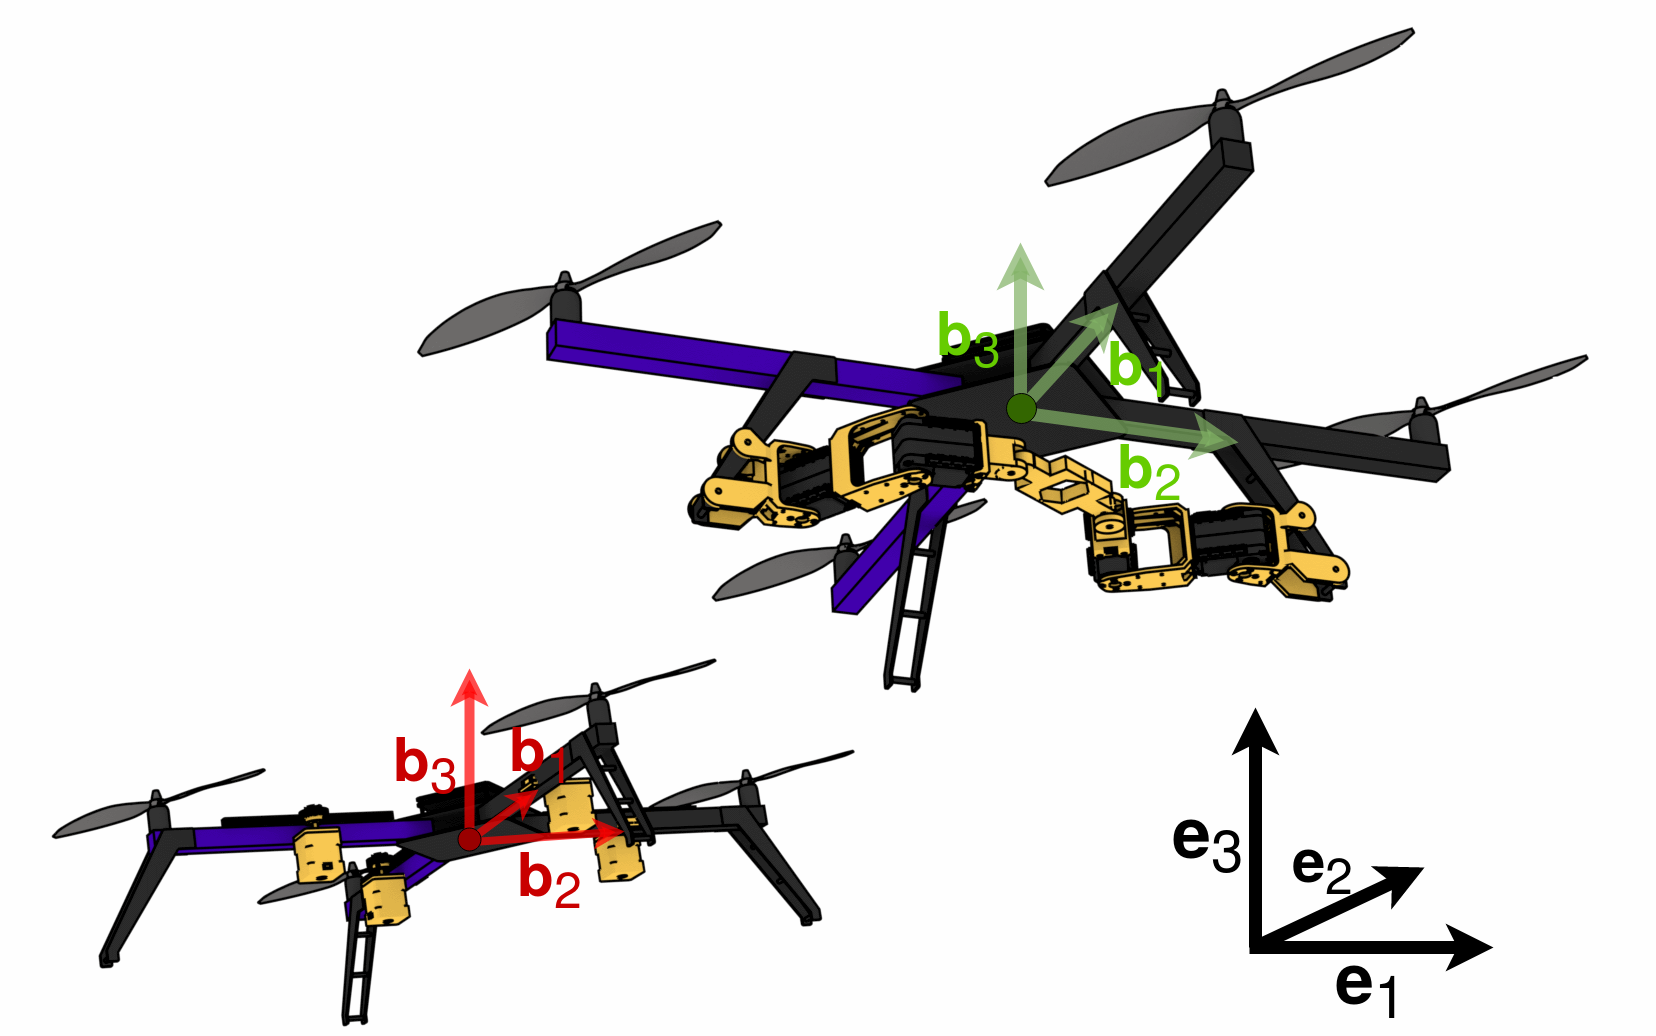
\includegraphics[width=\columnwidth]{pictures/uav.png}	
	\centering
	\caption{UAV model with MMC (left) and two 2-DOF overactuated manipulators (right) along with their respective coordinate systems. The manipulator end effectors are placed diametrically opposite from each other.}
	\label{fig:uav_model}
\end{figure}
\noindent Equations \eqref{model2}, \eqref{model3} and \eqref{model4} describe the dynamical flow of a rotating and translating rigid body in terms of evolution of $(\text{R},\textbf{x},\mb{\Omega},\dot{\textbf{x}})\in \text{TSE}(3)$ on the tangent bundle of SE(3). 

\indent Height and yaw of the UAV is controlled with variations in rotor velocity, whereas roll and pitch with variations in CoG. It is assumed that the first and the third propeller rotate clockwise, while the second and the fourth rotate counter-clockwise. The relation between moments, thrust and rotor velocity is the following:
\begin{gather}
	f_i = b_f \omega_{i}^2 \label{force}\\
	\tau_i = (-1)^i b_m f_i \, ,
\end{gather}
where the following terms are defined as:
\begin{itemize}
	\item $f_i \in \mathbb{R}$ - Thrust of the i-th motor
	
	\item $\tau_i \in \mathbb{R}$ - Moment i-th motor produces
	
	\item $b_f \in \mathbb{R}$ - Motor thrust constant
	
	\item $b_m \in \mathbb{R}$ - Motor moment constant
	
	\item $\omega_i \in \mathbb{R}$ - Rotation velocity of the i-th rotor
\end{itemize}
Total thrust can be expressed as:
\begin{equation}
	f = \sum_{1}^{4}f_i \, , \label{control:f}
\end{equation}
and total moment acting in the body-fixed frame as:
\begin{align}
	\begin{split} \label{control:M}
	\textbf{M} = [&m_{p}gd_x  \textbf{e}_1 \cdot \textbf{b}_{3,d} , \\
	&m_{p}gd_y \textbf{e}_2 \cdot \textbf{b}_{3,d}, \\
	&b_m(-f_1 + f_2 - f_3 + f_4)] \, ,
	\end{split}
\end{align}
where $d_x \in \mathbb{R}$ and $d_y \in \mathbb{R}$ are moving mass or payload offsets along x and y axis respectively. \\
Using \eqref{control:f} and \eqref{control:M} as control inputs of the system one is able to obtain the desired force of each rotor and the control offsets $d_x$ and $d_y$. While the control offsets are able to be directly applied as moving mass control inputs, in the manipulator case an additional transformation needs to take place. \\
Both manipulators are overactuated, meaning they have three actuators while operating in a 2-DOF workspace. They are placed in a diametrically opposite configuration as seen in \ref{fig:uav_model}, therefore only a single set of infinitesimal angle increments $\Delta q_1, \Delta q_2, \Delta q_3$ is sufficient as control input for both manipulators. \\
Conversion from payload offsets to angle increments is done using the inverse Jacobian of the manipulator end effector. Direct Jacobian matrix is presented as follows:
\begin{gather}
	\begin{bmatrix}
		d_x \\
		d_y
	\end{bmatrix}
	\, = \, 
	\Ja (q_1, q_2, q_3)
	\cdot 
	\begin{bmatrix}
		\Delta q_1 \\
		\Delta q_2 \\
		\Delta q_3
	\end{bmatrix} \\
	\Ja = 
	\begin{bmatrix}
		l_1\text{cos}(q_1) & l_2 \text{cos}(q_1 + q_2) & l_3 \text{cos}(q_1 + q_2 + q_3) \\
		l_1\text{sin}(q_1) & l_2 \text{sin}(q_1 + q_2) & l_3 \text{sin}(q_1 + q_2 + q_3) 
	\end{bmatrix} \, ,
\end{gather}
where $l_1$, $l_2$ and $l_3$ are the manipulator link lengths, while $q_1$, $q_2$ and $q_3$ are current actuator angles. Using Jacobian pseudoinverse, incremental update rule for actuator angles can be obtained as follows:
\begin{equation}
	\begin{bmatrix}
	\Delta q_1 \\
	\Delta q_2 \\
	\Delta q_3
	\end{bmatrix} 
	\, = \, \Ja^{-1} (q_1, q_2, q_3) \cdot
	\begin{bmatrix}
	d_x \\
	d_y
	\end{bmatrix}
\end{equation}
\\
Manipulator and moving mass actuator dynamics along with the change in desired rotor force is regarded as instantaneous while presenting the controller synthesis and stability conditions. However, within the Gazebo simulation environment, a certain transfer dynamic is taken into  account.